% This section provides the necessary context to help the reader understand the remainder of the thesis.

% Why this report is generated

The aim of this paper is to perform a data driven approach to extract relevant data to build machine learning classification model to detect specious company for a leading trade credit insurance provider. The trade credit insurance provides protection to the business (customer of the insurance company) in the event their buyers fail to pay for the products or services. Considering the raise of fraudulence business in recent past, the insurance provider has to monitor each buyers extensively before approving any insurance policy. Considering the number of number of policies are so high, a machine learning based recommended system was implemented for UK market to detect suspicious companies. Since the implementation of the system the solution saved around 1M pounds. Due to the success of the UK model, the organization decided to implement similar recommendation ending in other market.

For this paper, the a model focuses on identifying suspicious companies for Italian Market. Each country is fundamentally different in terms of trade credit policy. Hence, each country has its own internal process and method to identify the suspicious cases. To build the recommendation model below data driven machine learning strategies are used.

\mytodo{update terms: buyers, client and provider}

\subsection{Trade Credit Insurance}\label{subsec:trade-credit-insurance}
In business world trade credit is a regular practice done by manufactures, suppliers, and service providers to protect their financial interest from any types of risks.\mytodo{find the total yearly trade credit amount}. Companies sales their products and goods on credit to their buyers. Generally this is a continues process as back to back trade deals and payment happens between the suppliers and buyers. However, the amount of trade credit is very high, hence suppliers like to protect their interest by taking credit polices from financial institutions  \mytodo{cite what is trade credit}.

For financial institutions (credit insurance provider) ensures financial support to the supplier (client) in event of any mishaps. Trade credit is a risky business, hence before providing any insurance, financial institutions verifies both both supplier, sales, global economic conditions, external factors. As mentioned in section~\ref{sec: Intro}, due to the increased number of fraud cases, insurance providers have to also monitor fraudulent cases. Below are the types of fraud happens in the trade credit sector.

\begin{itemize}
    \item \textbf{Buyers Fraud:} When the buyers of the goods and products get benefited by not paying the dues to the suppliers.
    \item \textbf{Client Fraud:} When the clients of the insurance company, suppliers try to gain benefit by doing insurance fraud.
    \item \textbf{Joint Fraud:} When the suppliers and buyers cooperate another do conduct insurance fraud.
    \item \textbf{Internal Fraud:} When internal parties from the insurance company colludes with the client and conduct an insurance fraud.
\end{itemize}

In this study we will mainly focus on finding the suspicious buyers to prevent economic mishaps to protect the suppliers and the insurance companies from financial loss.


\subsection{Monitor Credit Policy}\label{subsec:monitor-credit-policy}


In the the figure~\ref{fig:trade_credit}, the process of trade credit issuance is shown.

\begin{figure}[htp]
    \centering
    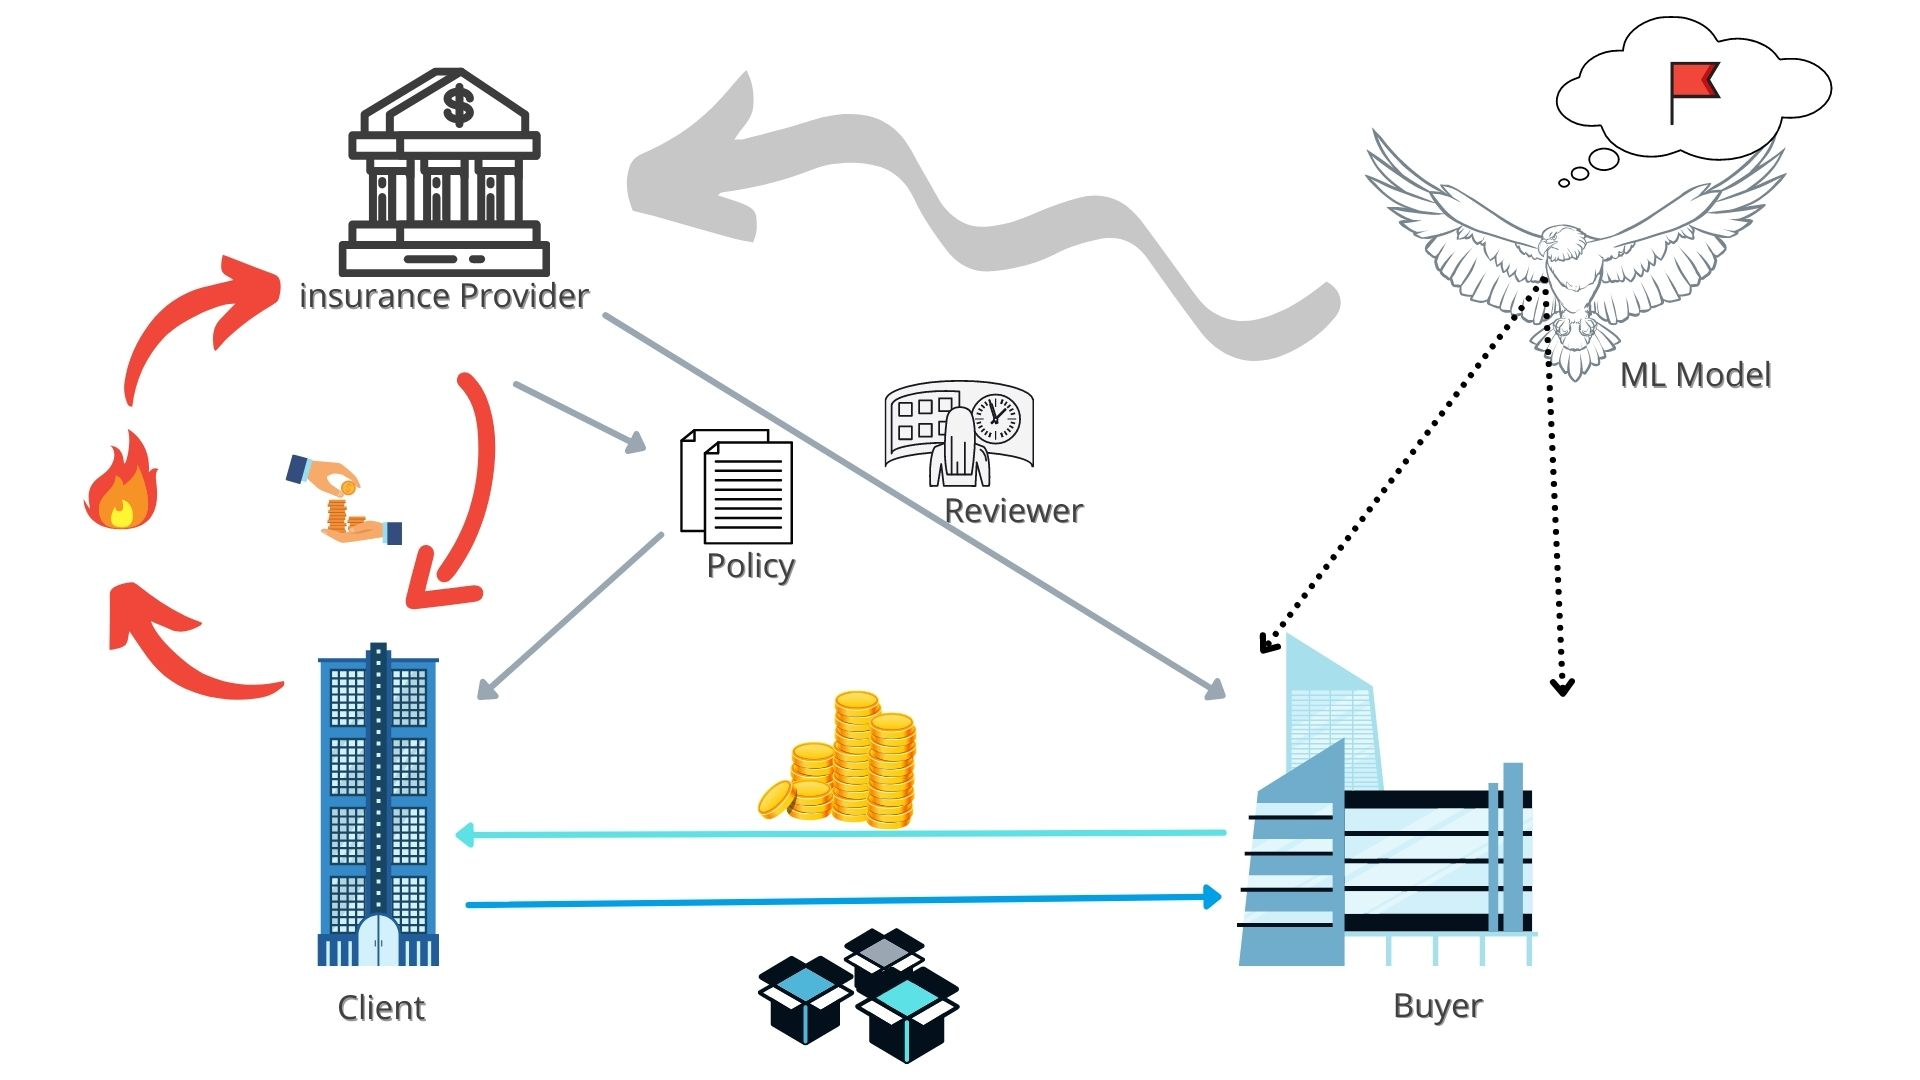
\includegraphics[width=\linewidth]{figures/monitor_buyers.jpg}
    \caption{Trade credit issuing process}
    \label{fig:trade_credit}
\end{figure}

\subsubsection{Traditional Approach}

\subsubsection{Machine learning base Approach}



